%!TEX root = ../../PhD_thesis__Edouard_Leurent.tex

\graphicspath{{2-Chapters/2-Chapter/}}

\chapter{Literature Review}
\label{chapter:2}

\begin{flushright}
	\begin{tabular}{@{}l@{}}
		\emph{Souhaite que la route soit longue. [\dots]}\\
		\emph{Visite aussi beaucoup de villes égyptiennes,}\\
		\emph{et n’aie de cesse de t’instruire auprès de ceux qui savent.}\\
	\end{tabular}
	
	Konstantinos Kavafis, \href{https://eleurent.github.io/sisyphe/texts/ithaki.html}{\emph{Ithaque}}.
\end{flushright}

\abstractStartChapter{}%
This chapter provides an overview of the sequential decision-making literature in the specific context of Autonomous Driving. It is meant to summarise the main directions that researchers have taken to tackle this wide problem, and discuss the questions that one practitioner may ask themselves when trying to apply \acl*{RL} to \acl*{AD}. Thus, I will prioritise breadth rather than depth, and remind the reader that each of these sections is not comprehensive and has been surveyed independently.
\minitocStartChapter{}

\section{Sequential decision-making}
\label{sec:sequential-decision-making}

\Cref{sec:scopes-and-challenges} presented the \acl*{RL} framework, that formulates the learning procedure as an optimal control problem. In this section, I start by recalling other design principles that have been considered for coming up with a good driving policy $\pi$.

\subsection{Motion Planning}

The development of motion planning techniques for intelligent vehicles dates back to the late 80s, supported by international research projects such as Eureka (1987) of the Prometheus program, followed by the DARPA Grand and Urban Challenges (2004, 2007), and more recently the VIAC (2010), GCDC (2011) and Delphi (2015) challenges. In two surveys \citep{Gonzalez2016,Paden2016} studying the literature of this period, three main approaches have been identified.

\paragraph{Search-based algorithms}

This method is based on a regular discrete partition of the state space $\cS$ called a \emph{lattice}, which must be connected by feasible trajectories \citep[\eg][]{Pivtoraiko2005}. This framing reduces motion planning to the problem of finding a shortest path in a known graph. Then, traditional graph-search algorithms such as Dijkstra's algorithm \citep{Dijkstra1959}, $A^\star$ \citep{Hart1968} or $D^\star$ \citep{Stentz1994} can been used to compute the optimal trajectory. This technique has been applied by at least five different teams during the DARPA Urban Challenge for driving on structured roads and unstructured parking: Dijkstra for team Ben Franklin \citep{Bohren2008} and VictorTango \citep{Bacha2008}, and $A^\star$ for Stanford University \citep{Montemerlo2008} and KIT \citep{Kammel2008}, and $D^\star$ by the winning team from CMU \citep{Urmson2008}. Kinematics constraints can also be included in the configuration graph, as in \citep[\eg][]{Latombe1991,Fraichard1993,Laumond1994}.

\begin{figure}[tp]
	\centering
	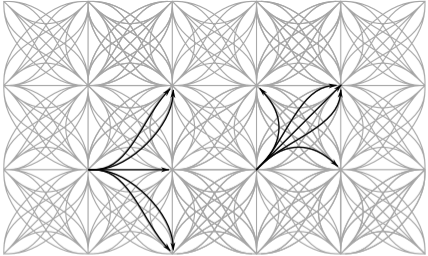
\includegraphics[width=0.5\linewidth]{img/lattice2}
	\caption{A lattice structure connects a discrete set of states by feasible trajectories}
\end{figure}

\paragraph{Sampling-based algorithms}

The limitation of search-based algorithms lies in the difficulty of formulating a regular lattice structure covering the states space $\cS$ with feasible transitions, and in the real-time constraint that may not be met by graph-search algorithms. To address them, sampling-based motion planners iteratively grow a set of reachable configurations by randomly sampling valid transitions. The most popular ones are \ac{PRM} \citep{Kavraki1996}, \ac{RRT} \citep{Lavalle98,Karaman2011} and \ac{MCTS} algorithms \citep{Coulom2006, Kocsis2006}. These methods have been used in the context of \acl*{AD} in \citep[\eg][]{Lamiraux2001,Sanchez2002,Lenz2016,Paxton2017,Faust2018}.

\paragraph{Optimisation-based algorithms}

The third approach consists in optimizing a parametrized trajectory with respect to a real-valued objective function. The most popular instance is interpolation between the current and goal states, which has been applied to various classes of functions in the context of Autonomous Driving, such as lines and circles \citep{Reeds1990}, clothoids \citep{Funke2012}, polynomials \citep{Xu2012}, and Bézier curves \citep{Gonzalez2016}.

These three approaches to motion planning thus rely on deterministic models of the vehicle dynamics. These models are often required to take a simple form so that the search or optimisation procedure can be solved efficiently, and other objects in the scene are often considered as static. In order to study more complex multi-agent interactions specifically, a collaborative approach to motion planning has been developed.

\paragraph{Cooperative planning}

The difficulty of predicting complex interactions patterns between multiple agents can be bypassed in one particular setting: cooperative motion planning for multiple vehicles. Indeed, the task of predicting how vehicles react to one another is replaced by the task of optimising the joint behaviour of all agents in the scene. As an effect, prediction outputs are replaced by input variables that can be chosen freely to maximise an objective function. Two main variations have been studied: coordination along fixed paths \citep{Altche2016,Altche2016b,Altche2017}, and general unconstrained motion planning \citep{LaValle1998}.
However, this framework does not allow to represent human behaviours, or more generally any behaviour that is not explained by the objective function. In particular, that lack of communication between agents and the resulting uncertainty lead to suboptimal, uncertain and multimodal trajectories that are not handled by cooperative planning approaches.


\subsection{Imitation Learning}
\label{sec:imitation-learning}

An orthogonal strategy to motion planning techniques is to learn a reactive policy $\pi(a|s)$ under supervision of an expert $\pi_E$ that produces a dataset $\cD$ of demonstration trajectories. To that end, a parametrized policy $\pi_\theta$ is optimised to minimise a regression loss $\cL$, for instance the $KL$ divergence to the expert actions distribution:
\begin{equation*}
\min_\theta \expectedvalue_{s\sim \cD} \left[\cL\left(\pi_{\theta}(a|s), \pi_E(a|s)\right)\right]
\end{equation*}
This approach is also referred to as behavioural cloning, and is particularly suited when only low-level high-dimensional inputs are available, such as camera images, which prevents access to the dynamics model required by motion planning approaches. 
The first application of imitation learning to autonomous driving is the ALVINN (Autonomous Land Vehicle In a Neural Network) project \citep{Pomerleau89}, where a 3-layer neural network was trained for the task of road following, as shown in \Cref{fig:alvinn}.
\begin{figure}[th]
	\centering
	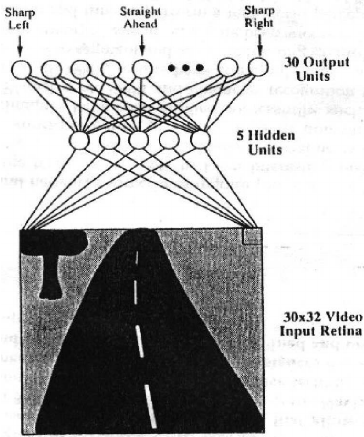
\includegraphics[width=0.4\linewidth]{img/alvinn}
	\caption{The 3-layer architecture used in ALVINN \citep{Pomerleau89}.}
	\label{fig:alvinn}
\end{figure}

\paragraph{Compounding errors} Unfortunately, the behavioural cloning paradigm is known to suffer from \emph{compounding errors}: since the future states depend on previous predictions (actions), the \iid assumption made in statistical learning does not hold. Therefore, small mistakes will place the system into states that are outside the training data distribution, as illustrated in \Cref{fig:compounding}, and resulting policies struggle to maintain high performances on long time horizons. This effect was identified and tackled in \citep{Ross2011}, who proposed to iteratively request expert labels (actions) from the states encountered by the current trained policy, rather than from the initial expert distribution. However, this can only be accomplished at the cost of a significant labelling effort. 
\begin{figure}[th]
	\centering
	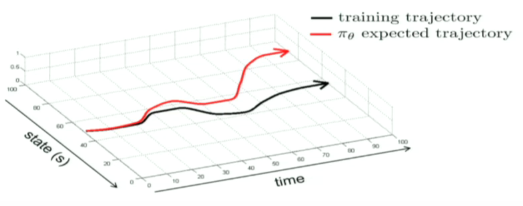
\includegraphics[width=0.7\linewidth]{img/cp4}
	\caption{As the agent deviates from the expert trajectories, the errors compound and push the agent further and further from the training distribution.}
	\label{fig:compounding}
\end{figure}
In the context of a Lane Keeping application, \citep{Bojarski2016} proposed instead to mitigate this issue during the data collection step by simulating deviations from the expert trajectories by means of two side cameras facing at the edge of the road. The corresponding synthetic expert controls were obtained by adding a constant adjustment term steer the vehicle back on track. The effect of compounding errors can also be delayed by further increasing the prediction performance, \eg by considering temporal dependencies as in \citep{Eraqi2017,Xu2017}. Other techniques than maximum likelihood estimation can be used to train the models, such as Generative Adversarial Imitation Learning \citep{Ho2016}, used for highway driving from range measurements in \citep{Kuefler2017,Bhattacharyya2018}.

\paragraph{Policy conditioning} A limitation of imitation learning for autonomous driving is fact that simply imitating human drivers by sampling likely trajectories is not sufficient: the sampling must also be conditioned on the current short-term destination specified by the Route planner. \citep{Codevilla2018} propose to achieve this by considering several policy heads for three possible behaviours when reaching an intersection: go straight, turn left or turn right. At test time, the appropriate policy is used at each intersection depending on the planned route. \citep{Rhinehart2020} present a more general approach that consists in learning a probabilistic model $q(s)$ of expert trajectories used as a prior, and inferring the maximum a posteriori trajectory given a test-time goal likelihood $p\parentheses{goal\mid s}$.

\subsection{Reinforcement Learning}

While the MDP framework undoubtedly consitutes a convenient theoretical framework for analysis, it may be too narrow a frame for the real world to fit in. In the sequel, by trying to cast the problem of Autonomous Driving as an MDP, we will identify multiple underlying assumptions that do not hold in practice, and relate them to existing research areas for which researchers proposed variants and solutions.

\section{States and partial observability}

\begin{figure}[th]
	\centering
	\begin{subfigure}[b]{.7\linewidth}
		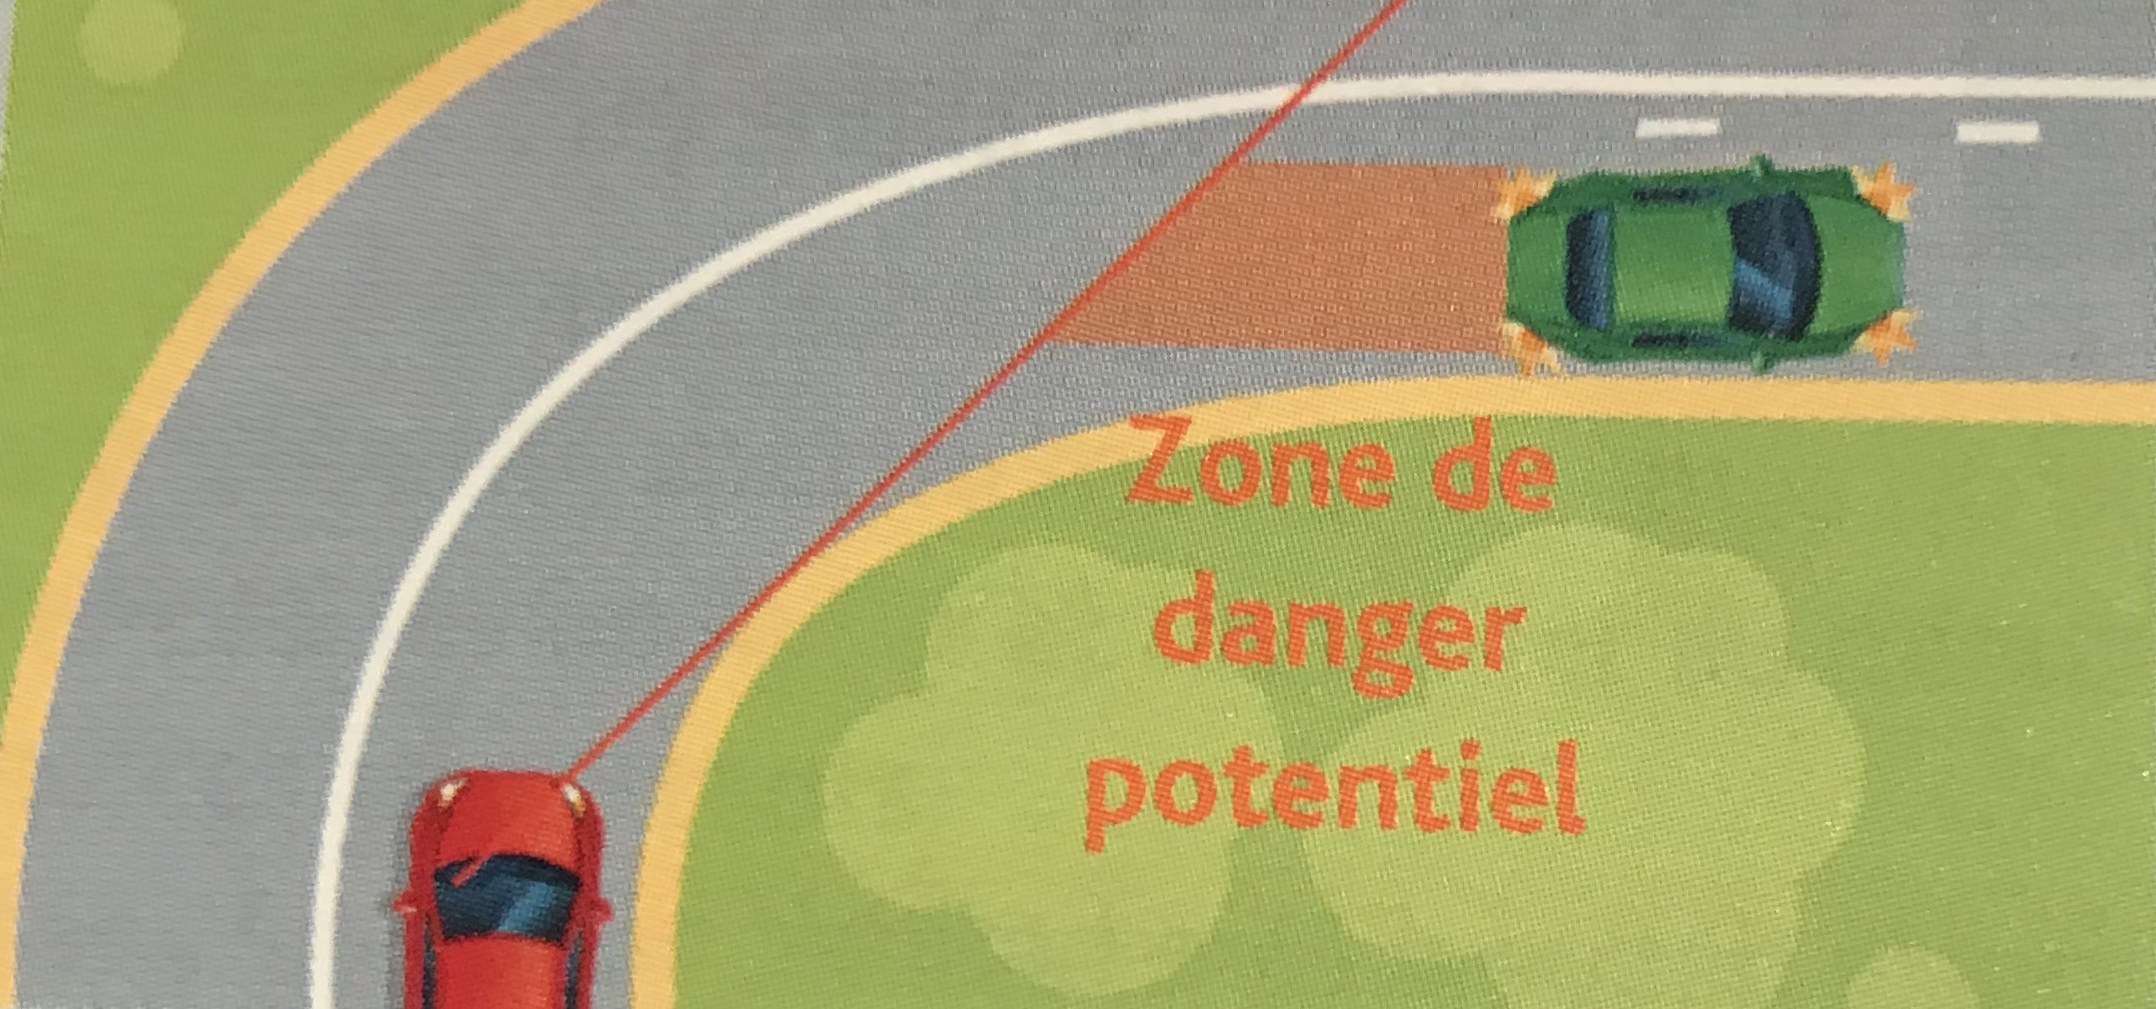
\includegraphics[width=\linewidth]{img/po-sensors}
		\caption{"Area of potential danger". A partial observability stemming from sensor occlusion in a turn.}
		\label{fig:po-occlusion}
	\end{subfigure}
	\begin{subfigure}[b]{.4\linewidth}
		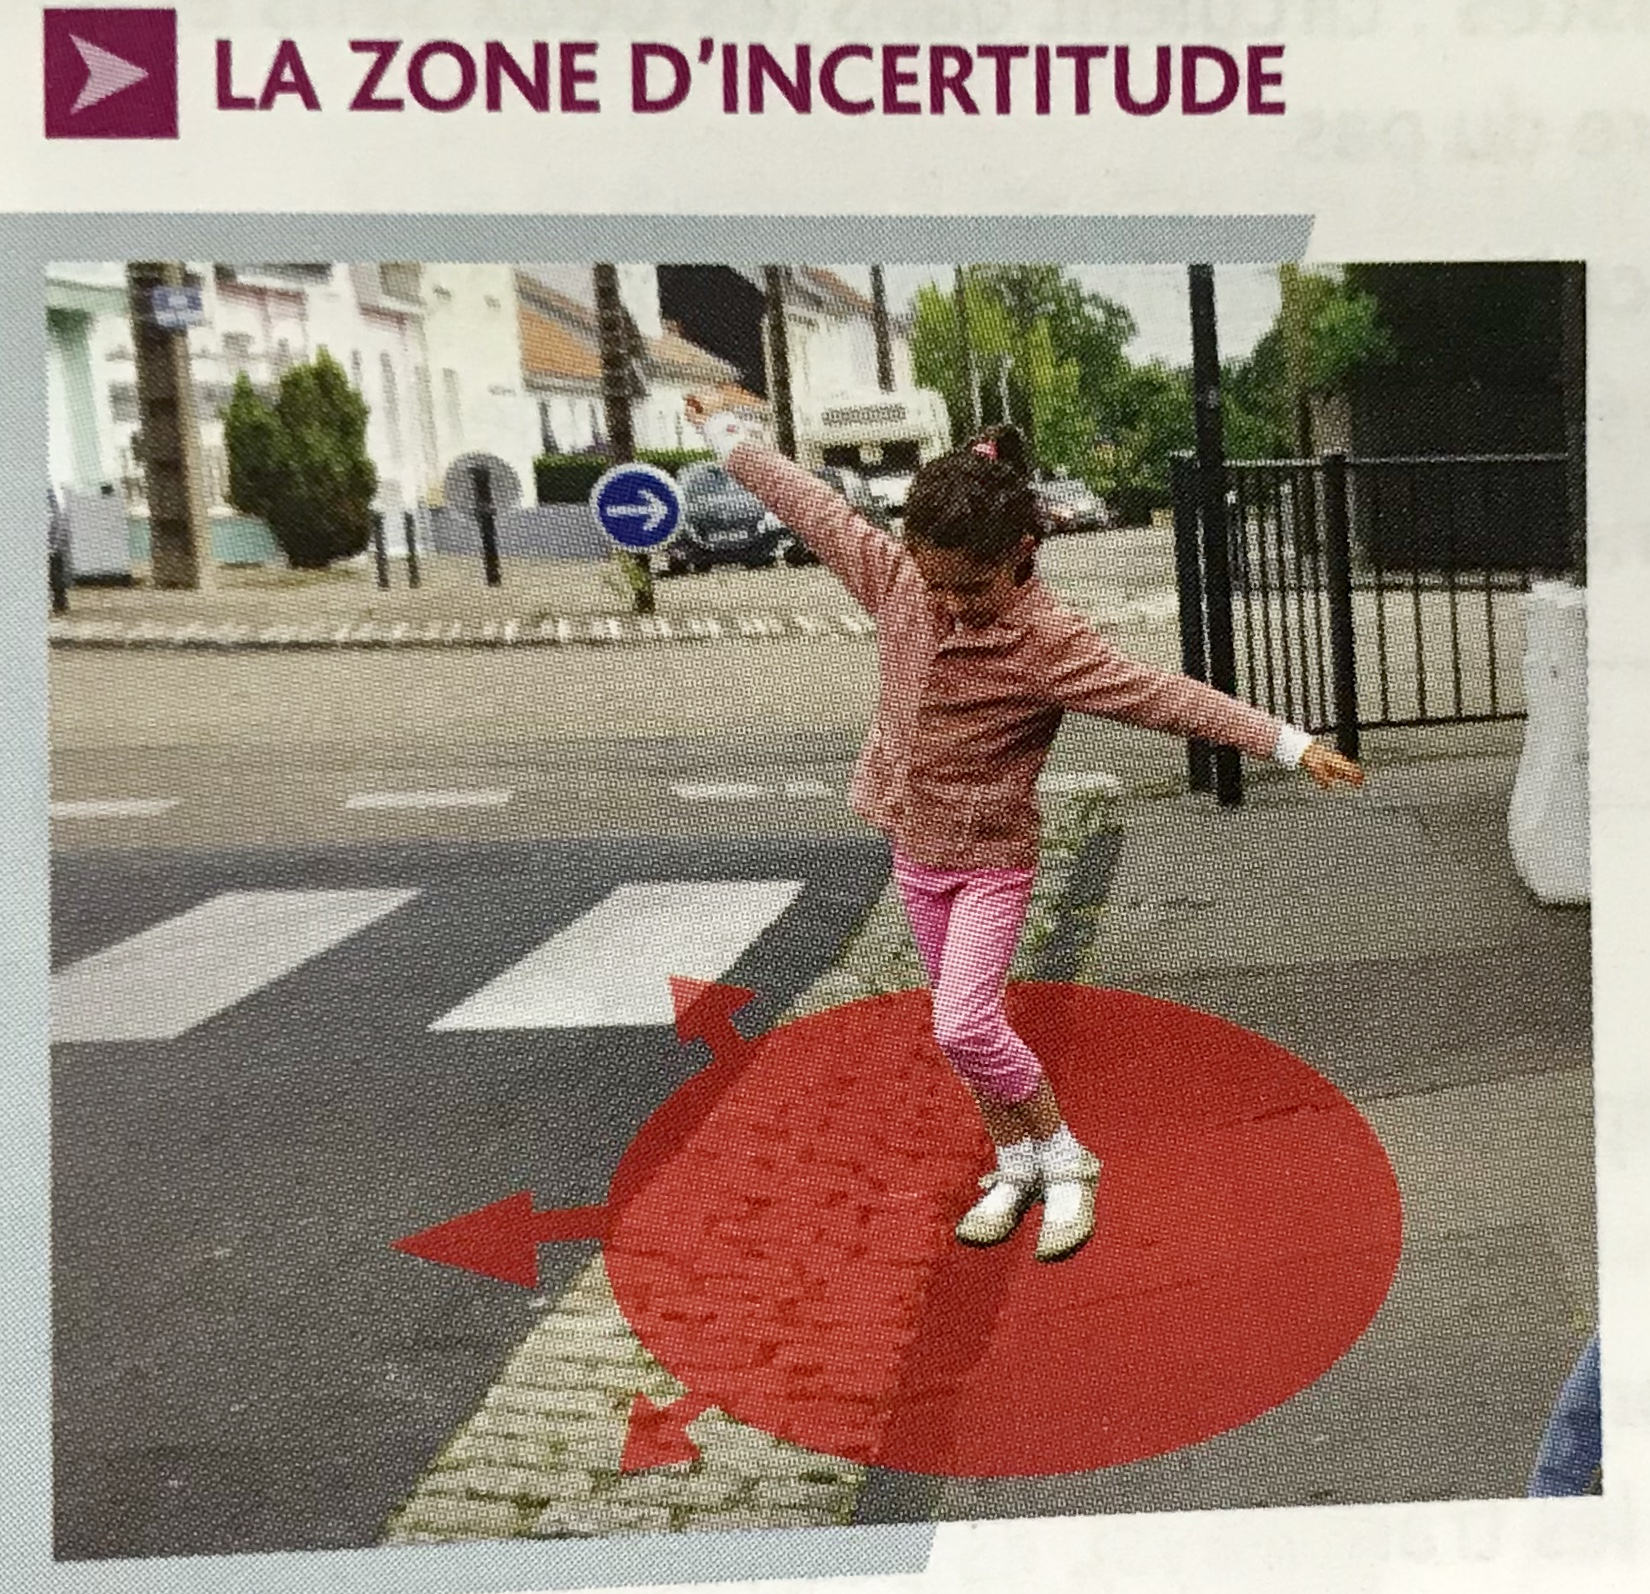
\includegraphics[width=\linewidth]{img/po-intentions}
		\caption{"Area of uncertainty". A partial observability stemming from unknown intentions of human agents.}
		\label{fig:po-intentions}
	\end{subfigure}
	\caption{Sources of Partial Observability in Autonomous Driving. Illustrations from \citep{ObjCode2017}.}
	\label{fig:partial-observability}
\end{figure}
\begin{figure}[th]
	\centering
	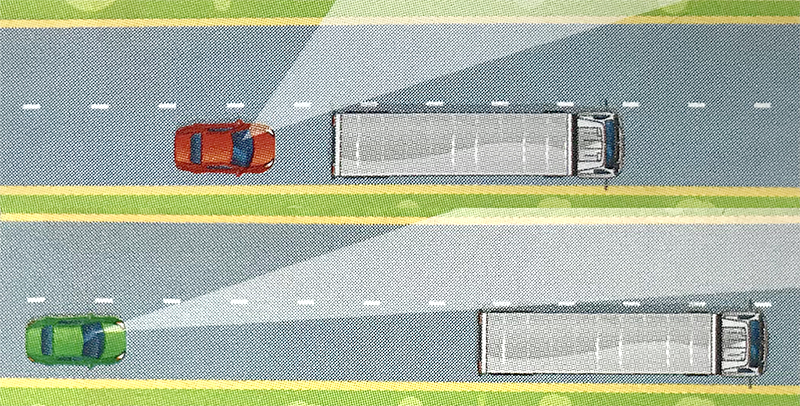
\includegraphics[width=0.7\linewidth]{img/pomdp}
	\caption{Information-seeking behaviours: the tailgating vehicle (top) should slow down, although it might decrease its immediate rewards, to gain valuable information in return (bottom). Image from \citep{ObjCode2017}.}
	\label{fig:information-seeking}
\end{figure}

In order to specify an MDP, the first step consists in defining the state space $\cS$, with the underlying assumption that the agent will have access its current state $s\in\cS$. Yet in practice, information about the scene can only be obtained through sensors, which produce typically noisy measurements \citep{Ulbrich2013,Du2010}. Worse, parts of the state may be missing altogether, as is the case when a scene entity is occluded by an obstacle \citep[\eg][]{Brechtel2013,Bouton2018,Sun2019}, as shown in \Cref{fig:po-occlusion}. To account for these difficulties, the concept of a \emph{Partially Observable} Markov Decision Process (POMDP) was introduced in \citep{Astrom1965}, extending the MDP framework with two additional quantities: an observation space $\Omega$, and an measurement model $O$ such that the observation $o\in\Omega$ is measured at state $s'$ with the conditional probability $O\parentheses{o\mid s',a}$. At each time step $t$, a belief $b_t\in\cM(\cS)$ over the state $s_t\in \cS$ is updated by performing Bayesian Filtering to compute the posterior state distribution:
\begin{equation*}
b_{t+1}(s_{t+1}) = \frac{O(o_t|s_{t+1}, a_t)\sum_{s_{t}\in\cS}P\parentheses{s_{t+1} \mid s_t, a_t}b_t(s_t)}{\sum_{s\in\cS} O(o_t|s, a_t)\sum_{s_{t}\in\cS}P\parentheses{s \mid s_t, a_t}b_t(s_t)}.
\end{equation*}
By conditioning the policy $\pi(a_t|b_t)$ on the belief $b_t$, the POMDP framework allows to optimally balance between information gathering and task completion, as shown in \Cref{fig:information-seeking}. However, there is a price to pay: the belief space $\cM(\cS)$ is much larger than the state space $\cS$ (\eg continuous of dimension $n$ when $\cS$ is finite of size $n$), which drastically increases the planning complexity. Exact solutions exist when $\cS$ is finite \citep{Pineau2003}, and approximate ones when it is compact \citep{Porta2006,Silver2010}. Even the belief update is intractable in general, when $\cS$ is compact. In the case of linear dynamics and Gaussian measurement noise, the belief update is known as Kalman Filtering \citep{Kalman1960}. It has been applied in \citep[\eg]{Bry2011,Bouton2017,VanDenBerg2017}, and in the context of quadratic costs --\ie the standard LQG problem-- which enables efficient computation of the optimal policy \citep[see e.g.][]{Xu2014,VanDenBerg2011}. The more complex observation model of sensor occlusions in continuous-space is handled in \citep{Brechtel2013,Brechtel2014,Bouton2018} where cautious driving policies are learned for crossing intersections; and in \citep[][]{Sun2019} where the observed behaviour of nearby vehicles is used to infer the presence of potentially occluded pedestrians.
Furthermore, the POMDP framework has been used to account for uncertainty in the intentions of other agents, as illustrated in \Cref{fig:po-intentions}. In \citep{Bandyopadhyay2013}, the authors propose a Mixed-Observability framework (MOMDP) in which the other drivers locations are observed but not their destinations. In \citep{Barbier2018}, the uncertainty lies in whether the other agents intend to yield of take the right of way. The value of inferring these drivers intentions has been assessed in \citep{Sunberg2017}, in comparison to MDP baselines where a static or maximul-likelihood behavioural model is assumed instead.



\section{Actions and temporal abstraction}

\begin{figure}[th]
	\centering
	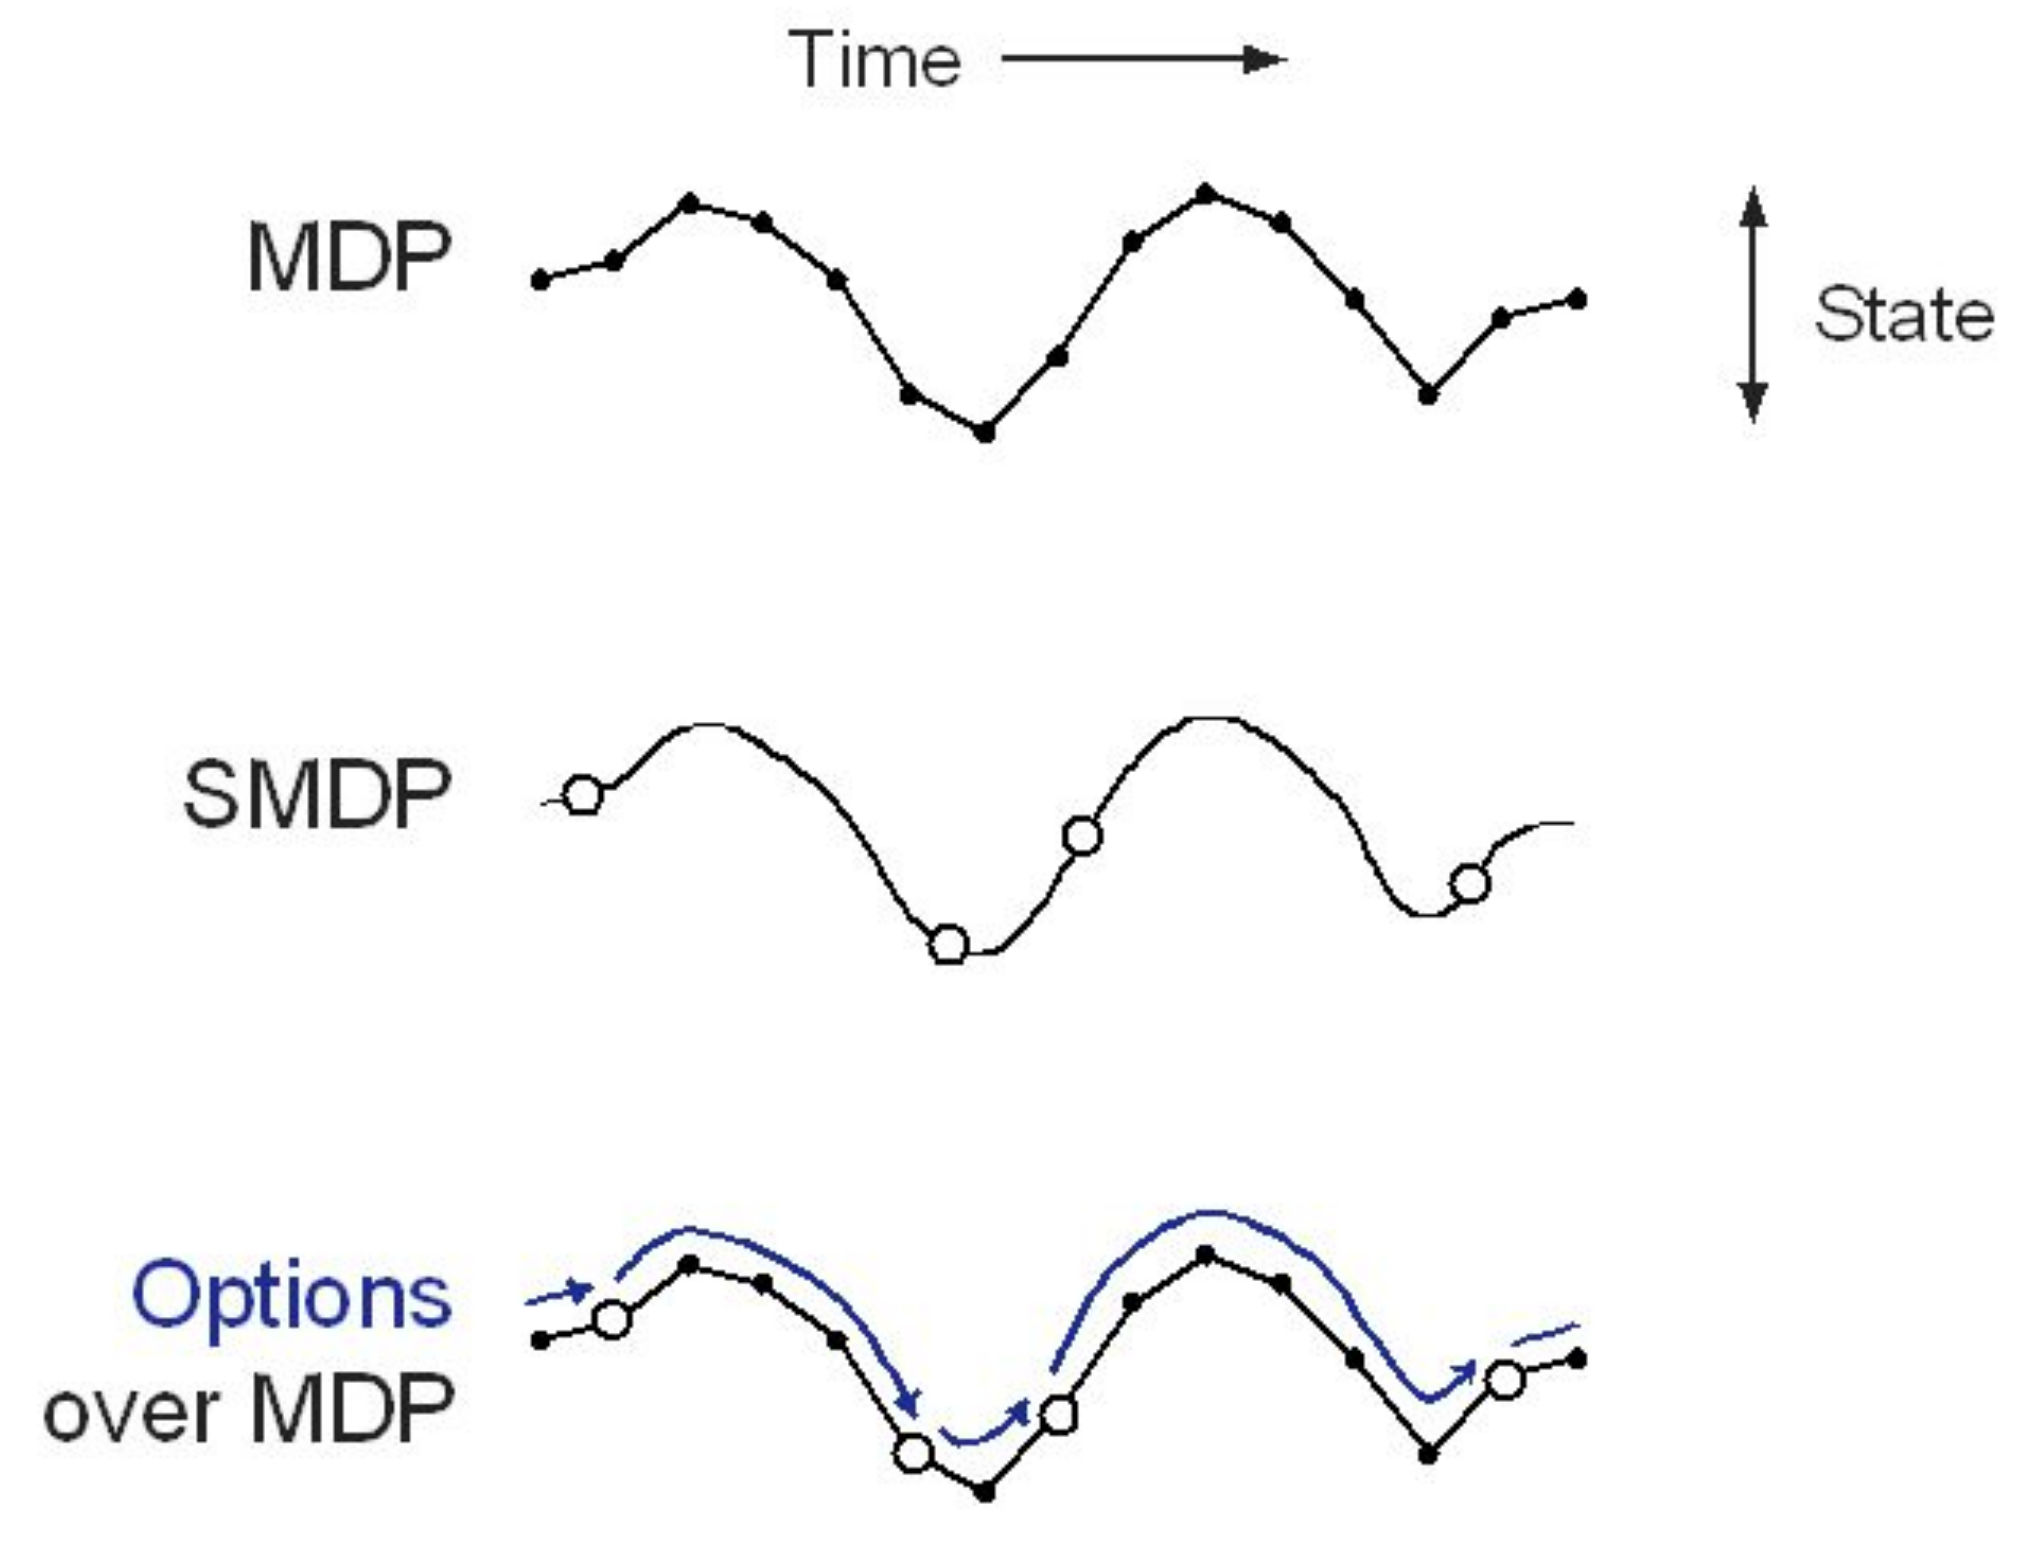
\includegraphics[width=0.5\linewidth]{img/smdp}
	\caption{Temporally extended sequences of actions can be used as skills, or \emph{options}, and futher used by a meta-policy to plan over long time horizons \citep{Sutton1999}.}
	\label{fig:smdp}
\end{figure}

The second step of when specifying an MDP is to choose an action space $\cA$. Suppose you are taking your first driving lesson, your instructor will be providing you with very detailed instructions about actuation such as: \emph{"turn the steering wheel by a full turn"}, \emph{"change gear"}, \emph{"brake smoothly"}, etc. After a few lessons however, the instructor will switch to more general instructions such as \emph{"change lane to overtake this vehicle"}, \emph{"yield to vehicles on the roundabout before merging"} or \emph{"drive slower in this area"}. And when, having finally got your driver's license, you start driving in an unfamiliar city, your friend in the passenger seat will merely give you directions: \emph{"follow the signs for the train station, and turn into the third street on the left"}. In short, driving involves reasoning at several time scales, and the corresponding decisions have different granularities. This can hardly be expressed in the MDP framework, where a single action space $\cA$ is considered. In particular, relying on shorter actions yields a smaller signal-to-noise ratio, which leads to slow learning when planning over long time horizon \citep{ShalevShwartz2017}. To address this issue, the concept of \emph{temporal abstraction} was introduced: nuclear actions $a\in\cA$ can be used to define temporally-extended \emph{skills} $\pi_o:\cS \rightarrow \cM(\cA)$, also called \emph{options}, which in turn can be used as meta-actions by a high-level \emph{option policy} $\pi(o|s)$. This idea is also referred to as \emph{Hierarchical Reinforcement Learning}, and was first analysed with the \emph{semi}-Markov Decision Process (SMDP) extension \citep{Sutton1999}, illustrated in \Cref{fig:smdp}. In autonomous driving, this hierarchy is typically imposed by the pipeline presented in \Cref{chapter:1}: Behavioural planning corresponds to the policy over options $\pi(o|s)$, while the low-level options $\pi_o$ are achieved in the Motion planning layer. However, this requires manually specifying the interfaces at each layer. For instance, in \citep{Barbier2018} a behavioural policy can only be trained after having defined a finite set of low-level skills, namely \emph{Stop}, \emph{Yield}, and \emph{Pass}. Consequently, using a fixed set of options constrains the exhaustivity of the set of option-policies, and may prevent recovering optimality if the architecture is not versatile enough. To bypass these limitations, \citet{ShalevShwartz2016} proposed to ensure sufficient exhaustivity of the class of available options by generating new options on-the-fly as paths in an option-graph, shown in \Cref{fig:options-graph}. Other works attempt to learn low-level skills jointly with the meta-policy \citep{Bacon2017,Vezhnevets2017,Heess2016}. In \citep{Paxton2017}, low-level skills such as \emph{follow} and \emph{overtake} are trained using Neural Networks and ad-hoc reward functions, while serving as meta-actions for a high-level tree-based planner.

\begin{figure}[th]
	\centering
	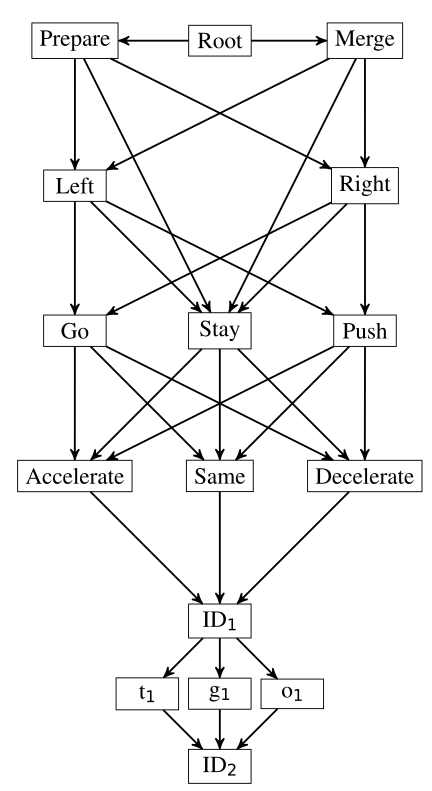
\includegraphics[width=0.3\linewidth]{img/options}
	\caption{A graph used to generate options \citep{ShalevShwartz2016}.}
	\label{fig:options-graph}
\end{figure}

\section{Rewards and inverse reinforcement learning}

Having defined the state and action spaces $\cS$ and $\cA$, we come to specify which state-action pairs are deemed \emph{desirable}, through the definition of the reward function $R$. Paradoxically enough, humans know how to drive but not necessarily how to explain their actions and justify why . A common approach to reward specification is colloquially known as \emph{reward engineering}, in which the reward function is parametrized as a linear combination of features $R(s,a) = \sum_i \omega_i \phi_i(s,a)$ . For example, such features may include the ego-vehicle speed, its longitudinal distance to a short-term goal, lateral distance to the lane centerline, or the presence of collisions.
By handling more and more use-cases, the number of features to consider will rise quickly, some of which contradicting each other. Then, the issue of how the properly choose the weights $\omega_i$ remains, and it can be increasingly hard to strike the right trade-off.
Besides, this difficulty is further exacerbated by an ambiguity lying in the blurry boundary between the reward function $R(s,a)$ and the value function $V(s)$. For instance, are safety distances desirable \textit{per se}, or only because respecting them means we are less likely to end up in an accident, which is the actual feature of interest here? Likewise, do road traffic regulation rules describe rewarding states or high-value states?

\begin{figure}[ht]
	\centering
	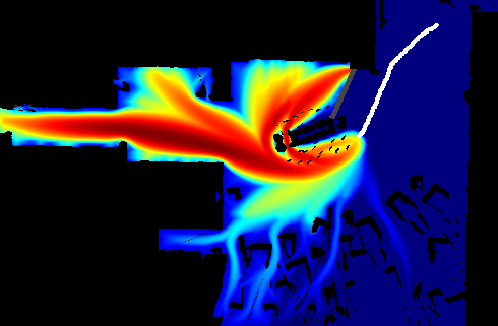
\includegraphics[width=0.7\linewidth]{img/pedestrian}
	\caption{Trajectory prediction for a pedestrian modelled as an optimal planner with a learned cost \citep{Ziebart2009}.}
	\label{fig:irl-pedestrian}
\end{figure}


One practical solution to these concerns is to iteratively refine the reward function $R$ until the corresponding optimal policy $\pi^\star$ matches the expected behaviour $\pi_E$ of human drivers. The careful or well-versed reader will have noticed that this approach is directly opposed to the \acl*{RL} problem, where the optimal behaviour $\pi^*$ stems from the reward function $R$. Accordingly, the aptly named \ac{IRL} framework aims at finding a reward function that makes the expert behaviour appear uniquely (near)-optimal. At first glance, this problem seems related to Imitation Learning formulation of \Cref{sec:imitation-learning} in its attempt to reproduce expert behaviour. This intuition is supported by the fact that \ac{RL} $\circ$ \ac{IRL} is the dual problem of state-action occupancy matching with respect to expert trajectories \citep{Ho2016}. Example applications of \ac*{IRL} to \acl*{AD} include the work of \citet{Kuderer2015} who learn the trade-off between comfort and efficacy in human lane-change trajectories. 

In addition to finding a good candidate reward for the ego-vehicle behaviour, \acl*{IRL} can also be applied for the purpose of predicting how other agents in the scenes are likely to behave, by modelling them as rational agents trying to maximise an unknown reward function to be learned. In that sense, \ac{RL} $\circ$ \ac{IRL} is a form of model-based \acl*{RL}.
For instance, this approach has been used to model of routing preferences of taxi-drivers \citep{Ziebart2008}, to predict the future trajectory of pedestrians \citep{Ziebart2009} as shown in \Cref{fig:irl-pedestrian}, and the behaviour of human drivers at an intersection \citep{Sun2019} or on a highway \citep{Sadigh2016}.


\section{Dynamics and transfer}

The last element of the \acl*{MDP} tuple.
Usually, no need to specify them: the dynamics are unknown, and only accessed by interaction.
But in the case of AD, this is not realistic.
Would require exploration, generating accidents, which is out of question.
 
How do we proceed?
Two ways: 
- offline RL
- simulation

But simulation-reality gap.
\citep{Pan2017,Liang2019}

Domain randomization: \citep{Tobin2017}

\section{Optimality criterion and safety}

Once the \acl*{MDP} is fully specified, the optimal policy maximises the expected return.
But is it an appropriate performance measure ?

A simple counter example

This has lead researchers and practitioners to consider alternative definitions of Optimality. Typically in critical settings, these approaches are are grouped under the name of \emph{Safe} RL.
Survey by \citep{Garcia2015}

\paragraph{Risk-sensitive Criterion}

Bandit / RL
\citep{Torossian19a} for risk optimization of stochastic blackbox functions.
Application to AD: \citep{Naghshvar2018} stationary object on the road, and highway ramp


\paragraph{Worst-case criterion}

Bandit / RL / Control theory:
Worst-case has been studied in the context of finite Markov Decision Processes with uncertain parameters by \citet{Iyengar2005}, \citet{Nilim2005} and \citet{Wiesemann2013}

\citep{Berkenkamp2015} with respect to the $\cH_2$ system norm.
H infinity control

Application to AD
\citep{Williams2018} TubeMPC for driving

\paragraph{Constrained Criterion}

In \citep{Berkenkamp2016}, blackbox optimization : and constraint is imposed during training.

CMDP optimization problem is to find a policy $\pi$ that maximizes $V^r$ subject to the constraint $V^c \leq \beta$

\citep{Altman1999,Achiam2017}

\citep{Tessler2019}: general constraints (discounted sums or average cost settings)

$$\max R \text{ s.t. } C \geq \beta$$

Applied to AD in \citep{Le2019}: two behavioral constraints: smooth driving and lane centering on CarRacing


\paragraph{Safe Exploration}

Constrain not the optimality definition but the exploration process: prevent error states through external knowledge (demonstrations, initial feasible policy).

\citep{Turchetta2016}: initial safe states and smoothness of the safety function : $r(s,a) > h$: explores the maximum reachable safe set without visiting unsafe states.

\citep{Koller2019}
additional model uncertainty under GP prior
given a safe controller, verify X and U polytopic constraints


This setting is questionable for AD, might be too restrictive: some standard states are prone to errors under adversarial behaviours, and cannot be avoided.
\citep{ShalevShwartz2017} instead defines a notion of Responsibility-Sensitive Safety.

\citep{Bouton2019}
\citep{Bouton2019workshop}: $P(reach goal |s, a) \geq \lambda$

\citep{leung2018infusing} HJI reachability
\citep{Fisac2019} HJI equation, non-convex constraints X,U
